%%%%%%%%%%%%%%%%%%%%%%%%%%%%%%%%%%%%%%%%%%%%%%%%%%%%%%%%%%%%%%%%%%%%%%%%%%%%%%%%
\section{TOKIO Framework} \label{sec:methods}
%%%%%%%%%%%%%%%%%%%%%%%%%%%%%%%%%%%%%%%%%%%%%%%%%%%%%%%%%%%%%%%%%%%%%%%%%%%%%%%%

\todo{We should shore up the description of all of this to the extent that we're presenting a framework with general components.
Then we describe our specific implementations.}

An end-user can't use this without escalated privileges so it should target facilities.
It is designed to facilitate post-mortem analysis.

The TOKIO framework is comprised of modular components 

We identified the following categories of ongoing instrumentation as being
critical to understanding both the I/O climate and I/O weather of a
production system.

\begin{figure}[t]
    \centering
    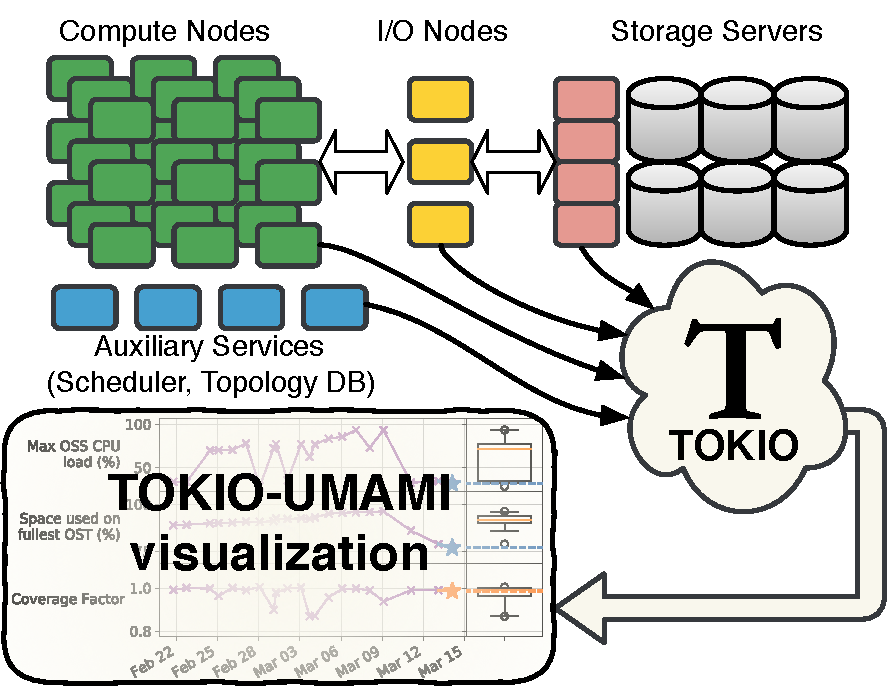
\includegraphics[width=\columnwidth]{figs/tokio-schematic.pdf}
    \caption{Overview of the TOKIO framework.  Data is collected from sources throughout the I/O subsystem, indexed and normalized, and then presented through an interface that relates I/O conditions during a specific job of interest to the overall climate of the I/O subsystem.}
    \label{fig:tokio-schematic}
\end{figure}

\subsection{Application behavior} \label{sec:methods/darshan}

Application behavior refers to the I/O pattern of a job as expressed from
the perspective of the application itself (i.e., the I/O pattern of the
application itself before any system-level optimizations are applied).
We rely on the Darshan I/O characterization tool~\cite{carns200924}
to capture this information.  Darshan transparently records concise,
bounded statistics about an application, such as the amount of time it
spent performing I/O, the distribution of access sizes, and what files
were accessed.  Reduction, compression, and storage of these statistics
is deferred until the application exits in order to minimize overhead.
Darshan has two notable properties that are desirable for use in TOKIO.
Because of its lightweight design, Darshan can be deployed for all
production applications on large-scale systems without perturbing
performance.  Because it operates at the application level, it is also highly
portable and can be deployed on nearly any major HPC platform.

\subsection{Storage system traffic}

Storage system traffic refers to the aggregate system-wide I/O workload
observed by the primary storage system.  On most modern-day HPC systems this
is reflected in the aggregate traffic that reaches the parallel file
system, and is most easily represented with ongoing time-series metrics.

\label{sec:methods/lmt}
The Lustre Monitoring Tool (LMT) is a widely used tool for Lustre file systems that collects Lustre-specific counters from \texttt{/proc/fs/lustre} on each Lustre OSS and MDS and presents them to external consumers via a MySQL database.
NERSC Edison implements LMT
as a part of the Cray Sonexion Lustre platform \cite{Keopp2014}, and we built
upon the pyLMT framework developed at NERSC \cite{Uselton2009} to preserve
server-side metrics during benchmark runs across all file systems evaluated.
These metrics include bytes read and written, CPU load averages, and metadata
operation rates on a per-server basis at five-second intervals.

\label{sec:methods/ggiostat}
We developed the \emph{ggiostat} tool in order to collect analogous data from
IBM Spectrum Scale (GPFS) file systems.  \assign{Zach}  It relies upon the
\texttt{mmpmon} monitoring system in GPFS to retrieve metrics from server and
client clusters.  These metrics are queried on five second intervals by a
persistent monitoring daemon and stored in an IBM DB2 database.
The metrics collected include bytes read and written,
read and write operations, and number of inode updates \todo{(is this
a proxy for metadata operation rates?)}. \todo{we should decide if we call it GPFS or IBM Spectrum Scale from here on out}

\subsection{Health monitoring \assign{Glenn and Kevin}}
\label{sec:methods/health}

Health monitoring refers to the current fault status and capacity of the
storage system: what components are offline, and how much storage space
remains on the available components.

% lfs df
% lctl dl -t
% mmlsdisk
% mmdf
For Lustre file systems, we record the fullness of each Lustre object storage target (OST) every fifteen minutes and associate the last measurement to precede the start of a job with that job.
We also record the server to which each target is mapped at this time, allowing us to identify object storage servers that are the recipient of failed-over OSTs.
On GPFS, we record the fullness of each disk LUN that contains data and the failure status of each LUN at the start of each job.
These data are then associated with job in which the collection was triggered.

\subsection{Job scheduling \assign{Glenn and Kevin}}

Job scheduling refers to the mix of concurrent application jobs that are running on the compute resources of a system at any given time.
Since I/O contention is often the result of other jobs running concurrently with a job of interest, we record the total number of jobs that were in flight at any point during the execution time of each job.
On the Edison system, this is accomplished by querying the Slurm job accounting logs for all jobs with a start time before the job of interest's end time and an end time after the job of interest's start time.
The job accounting data on Mira is uploaded by Cobalt into a database that can
be accessed via a python API call Ni. The API allows pulling out a list of
jobs for a given time range and running on a specific resource.
\todo{We can also determine overlapping jobs' I/O behaviors by associating their darshan logs via Cobalt (and IOminer), but we didn't do this here.  worth mentioning?}

%%%%%%%%%%%%%%%%%%%%%%%%%%%%%%%%%%%%%%%%%%%%%%%%%%%%%%%%%%%%%%%%%%%%%%%%%%%%%%%%
\section{Data integration}
%%%%%%%%%%%%%%%%%%%%%%%%%%%%%%%%%%%%%%%%%%%%%%%%%%%%%%%%%%%%%%%%%%%%%%%%%%%%%%%%

% \todo{PHC: fill this in.  Maybe it comes after experimental platforms?  At
% any rate, say something, even if brief, about how we bring together all of
% the instrumentation sources we listed into a coherent data set.}

The metrics outlined above are all integrated by the TOKIO framework by indexing the measurements from each data source discussed in Section \label{sec:methods} by time.
Starting with a job's Darshan log, which contains a job start and end time, scalar measurements such as concurrent job count and file system fullness are joined directly to the Darshan counters.
Timeseries data such as that provided by LMT and ggiostat are both reduced into scalar values (for example, as minimum, maximum, average) as well as retained as time-resolved slices which are indexed using the job identifier stored in the Darshan log file.

This data structure is very concise and can be represented as a simple index of pointers to the raw files in which each I/O system component stores its measurements (e.g., Darshan logs or pyLMT HDF5 files).
When transferring data between systems, all scalar measurements associated with a job can be serialized as a single row in a relational database or CSV-formatted file, and timeseries data can be encoded in a portable binary format such as HDF5.

For the purposes of the analyses performed in this work, all TOKIO-ABC data was aggregated and indexed on system (Mira or Edison), application, I/O motif (as described below and in Table \ref{tab:bench-config}), and whether the application primarily read or wrote its data. \todo{Should we make mention of the artifacts appendix and the data formats therein?}

\todo{everything below}

What were the challenges in doing the data integration, and how did we solve them?

\begin{itemize}
    \item get time synchronized everywhere via NTP
    \item add lustre topology to Darshan
    \item standardize on 5-sec intervals
\end{itemize}

Writing scripts that wedge native data formats into a format ingestible by an analysis tool is easy; the hard part is developing the analysis tools (which we did).

So it's not hard to ask readers to convert their existing instrumentation to a format which TOKIO can ingest.

Comment that not all systems have every metric

%%%%%%%%%%%%%%%%%%%%%%%%%%%%%%%%%%%%%%%%%%%%%%%%%%%%%%%%%%%%%%%%%%%%%%%%%%%%%%%%
\section{Experimental Methods} \label{sec:platforms}
%%%%%%%%%%%%%%%%%%%%%%%%%%%%%%%%%%%%%%%%%%%%%%%%%%%%%%%%%%%%%%%%%%%%%%%%%%%%%%%%

To demonstrate the utility and generality of the TOKIO framework, we deployed it on two distinct computing platforms.
We also assembled a suite of I/O benchmarks, called the TOKIO Automated Benchmark Collection (TOKIO-ABC), to run on these two systems and explore the utility of TOKIO.  
Over the course of a month-long evaluation period, we collected measurements from the data sources described in \ref{sec:methods} and used these data to contextualize the performance variability observed in the daily TOKIO-ABC tests.
In this section, we describe the configuration of the TOKIO-ABC tests and the platforms on which TOKIO and TOKIO-ABC were deployed.

\subsection{I/O performance regression tests} \label{sec:methods/tests}

% abandon all hope ye who try to edit this stupid table by hand.  I used
% http://www.tablesgenerator.com to make it.
\begin{table*}[h]
\centering
\begin{tabular}{|c|c|c|c|c|c|c|c|}
\hline
\multirow{2}{*}{\textbf{Benchmark}}                    & \multirow{2}{*}{\textbf{I/O Motif}}                           & \multicolumn{3}{c|}{\textbf{Mira}}                        & \multicolumn{3}{c|}{\textbf{Edison}}                      \\ \cline{3-8} 
                                                       &                                                               & \textbf{\# Nodes} & \textbf{\# Procs} & \textbf{\# Bytes} & \textbf{\# Nodes} & \textbf{\# Procs} & \textbf{\# Bytes} \\ \hline
IOR                                                    & \begin{tabular}[c]{@{}c@{}}MPI-IO\\ shared file\end{tabular}  & 1,024             & 16,384            & 1.0 TiB           & 128               & 2,048             & 0.5 TiB           \\ \hline
IOR                                                    & \begin{tabular}[c]{@{}c@{}}POSIX\\ file per proc\end{tabular} & 1,024             & 16,384            & 1.0 TiB           & 128               & 2,048             & 2.0 TiB           \\ \hline
HACC                                                   & \begin{tabular}[c]{@{}c@{}}GLEAN\\ file per proc\end{tabular} & 1,024             & 16,384            & 1.5 TiB           & 128               & 2,048             & 2.0 TiB           \\ \hline
\begin{tabular}[c]{@{}c@{}}VPIC\\ BD-CATS\end{tabular} & \begin{tabular}[c]{@{}c@{}}HDF5\\ shared file\end{tabular}    & 1,024             & 16,384            & 1.0 TiB           & 128               & 2,048             & 2.0 TiB           \\ \hline
\end{tabular}
\caption{TOKIO Automated Benchmarking Collection (TOKIO-ABC) benchmarking configurations}
\label{tab:bench-config}
\end{table*}

The passive instrumentation methods described in Section \ref{sec:methods} are essential for ongoing understanding production workloads, but they do not provide any fixed reference point:
the workload and state of the system evolves over time.
We must therefore incorporate
routine, formalized I/O performance regression tests in order establish baseline behavior.

We developed the TOKIO Automated Benchmark Collection to meet
this need.
TOKIO-ABC consists of a collection of benchmarks, including
both synthetic and application-derived workloads, that can be scaled in
both the number of processes and data volume according to the constraints
of the system on which it is deployed.
Our two goals in choosing a scale for TOKIO-ABC deployment were
a) to saturate the storage system and
b) to limit core-hour consumption sufficiently for daily execution.
We use
a collection of benchmarks because performance is not well-represented
by a single benchmark result; each storage system has its own strengths
and weaknesses for different workloads.  The collection of benchmarks is
executed within a job script that can be scheduled nightly by a continuous
integration system or cron job.  The script insures that no more than
one TOKIO-ABC instance is active at a time, and all benchmark results
and Darshan logs are archived for analysis at the conclusion of the job.
The initial set of benchmarks included in TOKIO-ABC are as follows:

\begin{itemize}
\item \textbf{HACC} \assign{Shane}
\item \textbf{VPIC} 
Vector particle-in-cell (VPIC) is a highly scalable code developed to simulate
interactions among trillions of plasma physics particles  \cite{Bowers2008}.
VPIC-IO kernel extracts the I/O operations of a magnetic reconnection
simulation, where each MPI process writes 8M (i.e., $8 \times 1024 \times 1024$) particles. Each
particle has eight properties (six floating point and two integer) and each
property is a single dimension array. The total number of particles depends on
the number of MPI ranks used. The kernel uses the H5Part API \cite{H5Part} to write
the data to a single shared HDF5 file, and the execution of the I/O kernel includes
creating and opening a file, writing data to the file, and closing the file.

\item \textbf{BD-CATS} The BD-CATS clustering system~\cite{Patwary2015}  represents
one of the analyses that is commonly performed on the output of VPIC's particle data files.
For this study, we emulate the I/O workload of a clustering both particle
positions and momenta in three dimensions using the BD-CATS-IO I/O kernel benchmark.  This amounts to 75\% of the data
contained in the HDF5 file (generated by the VPIC-IO kernel) being read.

\item \textbf{IOR} The IOR benchmark has been used extensively
to characterize the performance characteristics of parallel file systems\cite{Yildiz2016,Xie2012,Lofstead2010,Uselton2010}
due to its extensive configurability.  For the purposes of this work, we applied
IOR to determine each file system's performance variability under conditions
where an application is performing I/O using the ideal parameters for each
file system.

\end{itemize}

%%% GKL - the following Edison description is very wordy.  Would this be better in a table?
\subsection{NERSC Edison} \label{sec:platforms/edison}

Edison is a Cray XC-30 system deployed at the National Energy Research Scientific Computing Center (NERSC) and is comprised of 5,586 compute nodes each with two 12-core Intel Xeon E5-2695 v2 processors and 64 GiB DDR3-1866 DRAM.
It has three Lustre-based parallel file systems implemented in Cray Sonexion 1600 appliances; two of the file systems are identically configured with users given a scratch directory on one or the other, while the third is reserved for users with specific parallel I/O requirements.

Edison's scratch1 and scratch2 file systems are identically configured with 24 Lustre object storage servers (OSSes), each with a single declustered RAID object storage target (OST).
These two file systems each have a total capacity of 2.2 PB and are capable of 48 GB/sec, and users are evenly distributed across these two file systems such that user diversity and I/O workloads should be similar on both.
However, Edison's scratch3 file system has 36 OSSes, 36 OSTs, 3.3 PB of capacity, and 72 GB/sec of peak performance, and users requiring high parallel bandwidth must specifically request access to receive an allocation on it.  Thus, the scratch3 file system should be biased towards larger, more coherent I/O traffic than the other two Edison file systems.

The Edison architecture routes I/O traffic from the Cray Aries high-speed network to the InfiniBand storage fabric through LNET-based I/O nodes.
The scratch1 and scratch2 file systems each have nine LNET I/O nodes through which all of their traffic is routed via Lustre fine-grained routing, and the scratch3 file system uses thirteen LNET routers.
As a result of this design, all of Edison's I/O traffic that is bound for one file system shares the same subset of LNET routers on Edison, but this also ensures that Lustre traffic for one file system does not contend for bandwidth with other file systems' I/O nodes.

The TOKIO-ABC benchmark input configurations for Edison described in Table \ref{tab:bench-config} were sized to achieve a high fraction of peak I/O bandwidth for each file system, and indeed, the IOR benchmark configurations demonstrated peak performance at 90\% of the aforementioned file system maximum.
\todo{Describe how many OSTs we used}

\subsection{ALCF Mira} \label{sec:platforms/mira}

\assign{Phil} Mira is an IBM Blue Gene/Q system deployed at the Argonne Leadership Computing Facility (ALCF) and is comprised of 49,152 compute nodes, each equipped with a 16-core PowerPC A2 processor and 16 GiB of DDR3 DRAM. The 48K 
compute nodes are connected to 384 I/O nodes for a ratio of 128 compute nodes
to each I/O node. The I/O node is identical hardware to the compute node,
except that it has a single Infiniband QDR link to the storage fabric.
Mira has two primary GPFS-based parallel file systems using DDN SFA12Ke storage appliances.
Both of these file systems, mira-fs0 and mira-fs1 share the same
Infiniband QDR fabric. Although jobs running that use mira-fs0 may not compete
for storage hardware resources, they will still compete for SAN resources.
The allocation used for this project has space allocated on mira-fs1 so it 
was the target of this study.
The mira-fs1 file system has 48 network shared disk (NSD) servers with each of the
servers managing 7 SATA RAID6 LUNs and 0 or 1 SSD RAID 10 LUNs. The GPFS metadata
is placed on the SSD LUNs while data is placed on the SATA LUNs. The volume provides a total of 7 PB of storage, and it is capable of delivering an aggregate bandwidth of 90 GB/sec peak performance.

% \subsection{Mira benchmark configuration} \label{sec:platforms/mirabenchmarks}

For the selection of the job size for the test framework on Mira, we had to
base our choice on the number of compute resources rather than the saturation of
I/O subsystem.
Mira's I/O architecture is fundamentally different from that of Edison in that it has fixed-size partitions of compute nodes connected to each I/O forwarding node.
Saturating the I/O bandwidth of the underlying storage servers requires the
use of many I/O nodes, meaning that peak storage bandwidth can only be
attained using a large portion of the system's available compute nodes.
Running daily I/O benchmarks that span a large portion of Mira's compute
nodes is impractical due to the lengthy queue times of capability jobs and
the disruption this would have to job scheduling.

For these reasons, we decided to use 1,024 Mira compute nodes (a single
rack), a partition size that was small enough to move quickly through
scheduler queues but large enough to exercise an adequate portion of the
storage system.  This job size corresponds to eight I/O nodes, each with a QDR 4x InfiniBand link to the SAN, totalling an absolute peak of ~25 GB/sec.
In practice, the TOKIO-ABC IOR configuration for Mira listed in Table \ref{tab:bench-config} was able to achieve 80\% of the absolute peak performance of this I/O node allocation.
% highest IOR was 20351.604001 MiB/sec (or MB/sec?? what's the darshan-parser --perf unit?)

%%% GKL - following is already stated in table
% We use 16 processes per node, resulting in a total of 16,384
% processes executing each benchmark. The benchmark workloads were configured
% to use enough I/O volume to drive the storage system for 1--2 minutes.
